\documentclass[journal]{IEEEtran}

\usepackage{graphicx}
\usepackage{cite}
\usepackage[hidelinks]{hyperref}  % Disable link colors

% Title and author information
\title{Innovative Applications of Generative AI in Dynamic Semantic Content Generation for Semantic Communication Systems}

\author{Xianzhe~Li,~\IEEEmembership{Student ID:~2022214880} 
\thanks{Xianzhe Li is with the International College, Chongqing University of Posts and Telecommunications, Chongqing, China (email: 2022214880@stu.cqupt.edu.cn).}
}

% The paper headers
\markboth{Academic  English Writing , CQUPT, 2024~Fall}%
{Li: Innovative Applications of Generative AI in Semantic Communication Systems}

\begin{document}

% Make title area
\maketitle

\begin{abstract}
This paper explores the potential of Generative AI (GAI) in enhancing semantic communication systems by facilitating dynamic semantic content generation. The study investigates how GAI-driven systems can optimize semantic encoding and decoding processes to enable efficient, adaptive communication across varied real-world applications, such as autonomous driving and smart cities. By dynamically generating context-aware content, GAI-driven semantic communication systems can achieve better bandwidth utilization and resource allocation, thereby addressing the complex communication needs of real-time, high-demand environments.
\end{abstract}

% Keywords
\begin{IEEEkeywords}
Generative AI, Semantic Encoding, Adaptive Decoding, Resource Optimization, Real-Time Applications
\end{IEEEkeywords}

\IEEEpeerreviewmaketitle

\section{Introduction}
\IEEEPARstart{T}{he} rapid advancement in wireless communication has introduced new paradigms that move beyond traditional Shannon information theory, particularly through semantic communication, which focuses on meaning over bit reproduction \cite{9530497}. This study aims to examine how Generative AI (GAI) enhances the capabilities of semantic communication systems by enabling dynamic semantic content generation. Specifically, the paper discusses applications in semantic encoding and decoding for adaptive and context-sensitive communication in sectors like autonomous driving and smart cities.

Recent research in generative AI \cite{Radford2018ImprovingLU} and semantic communication networks \cite{10614204,10447237} suggests that combining these fields can yield highly adaptive and efficient communication systems that meet the requirements of next-generation networks, such as 5G/6G. The innovative applications explored in this study highlight GAI’s ability to handle complex data, adapt in real-time, and minimize bandwidth consumption \cite{liu2024semanticcommunicationsartificialintelligence}.

\textit{Contributions:} This study presents the following key contributions:
\begin{itemize}
    \item Analysis of GAI-driven semantic encoding and decoding mechanisms for adaptive communication.
    \item Examination of GAI’s role in enhancing real-world semantic communication systems.
    \item A review of resource optimization through dynamic, context-aware content generation.
\end{itemize}

% Insert the first image for Semantic Communication Benefits
\begin{figure}[htbp]
    \centering
    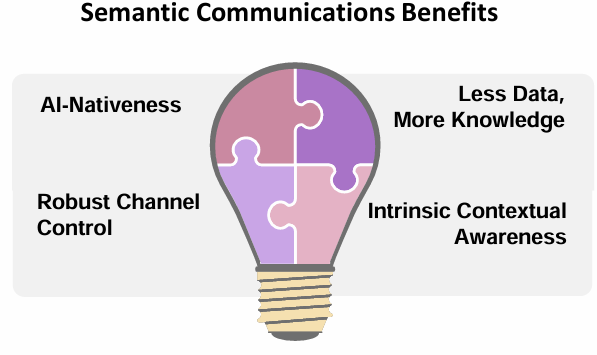
\includegraphics[width=\linewidth]{1.png}
    \caption{Illustrative figure showcasing the benefits of semantic communications.\cite{chaccour2022dataknowledgebuildinggeneration}}
    \label{fig:semantic_benefits}
\end{figure}

\section{Background and Related Work}

\subsection{Generative AI in Communication}
Generative AI has been widely studied for its ability to create contextually relevant content across different domains. The foundational work on generative pre-training by Radford et al. \cite{Radford2018ImprovingLU} laid the groundwork for content generation across numerous applications. In telecommunications, large generative models are being explored to reduce the need for task-specific training, thus promoting model generalization and efficiency \cite{bariah2023largegenerativeaimodels,10614204}.

\subsection{Semantic Communication}
Semantic communication, which focuses on conveying meaning rather than data accuracy, has emerged as a core component of next-generation networks \cite{9955312}. In scenarios like autonomous driving, efficient and adaptive communication becomes crucial, as semantic representations allow for resource-conscious message encoding and decoding \cite{10319661,raha2023generativeaidrivensemanticcommunication}.

\subsection{Combined Applications of GAI and Semantic Communication}
Recent works have started to explore how GAI can support semantic communication by optimizing message encoding and decoding \cite{10447237}. Studies suggest that GAI-driven systems could improve network efficiency through adaptive content generation and low-latency response times, essential for applications in intelligent transportation systems and smart city infrastructures \cite{jiang2024largeaimodelbasedsemantic}.


% Insert the second image for Synergistic relationship between SemCom and GAI
\begin{figure*}[htbp]
    \centering
    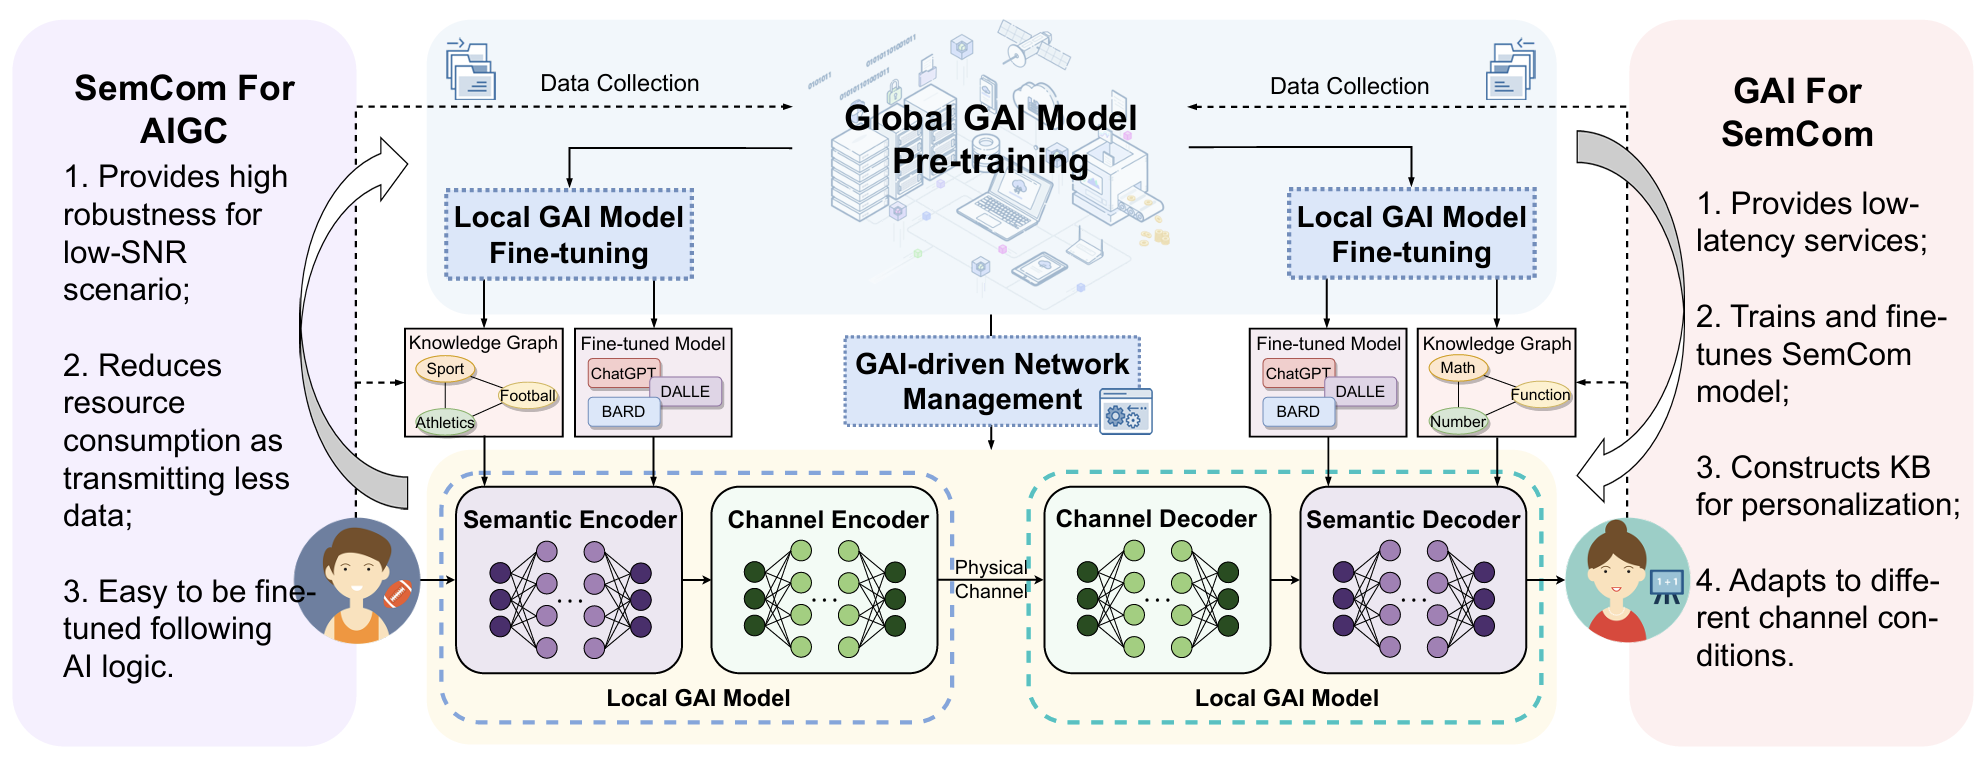
\includegraphics[width=0.8\textwidth]{2.png}
    \caption{The synergistic relationship between SemCom and GAI in SemCom-empowered AIGC transmission. The central part of the diagram depicts the framework for AIGC transmission, outlining the process from the cloud server to user devices. The left part highlights the contributions of SemCom to AIGC, and the right part details the advantages GAI offers to SemCom.\cite{10614204}.}
    \label{fig:synergistic_relationship}
\end{figure*}

\section{Methodology}

\subsection{GAI-Driven Semantic Encoding}
Generative AI (GAI) plays a crucial role in enhancing the efficiency of semantic encoding by transforming raw data into minimalistic, contextually rich messages that emphasize core meanings while eliminating redundancy. GAI leverages large AI frameworks that dynamically identify and extract only the most relevant information, tailoring the encoding to focus on semantic value rather than exhaustive data replication. This approach significantly reduces the required bandwidth and data transmission load, a critical factor in bandwidth-sensitive environments such as IoT and next-generation wireless networks \cite{chaccour2022dataknowledgebuildinggeneration}. For instance, by utilizing GAI-driven feature extraction, communication systems can minimize unnecessary data, focusing only on transmitting information that impacts the communication outcome, thereby optimizing resource allocation and improving transmission efficiency \cite{10634888,10614204}.

\subsection{Adaptive Decoding for Real-Time Applications}
In applications requiring real-time responsiveness, GAI models provide adaptive decoding capabilities that allow the receiver to interpret incoming messages dynamically based on contextual cues. This adaptive approach is essential in high-stakes environments such as autonomous driving, where rapid adjustments in message decoding are necessary for immediate decision-making. GAI enables systems to modify decoding strategies in real-time by leveraging contextual data from the surrounding environment, thereby enhancing the reliability and relevance of the communication \cite{10614204}. Such GAI-driven decoding processes allow the receiver to reconstruct semantically meaningful content even in scenarios where data distributions may vary or specific task requirements at the transmitter side are not predefined \cite{10447237}.

\subsection{Data and Resource Optimization Techniques}
Integrating GAI into semantic communication systems facilitates advanced resource management techniques that optimize data transmission and reduce overall communication overhead. Techniques such as generative adversarial networks (GANs) and diffusion models have been effectively applied to optimize the encoding and selective transmission of critical data. This process is especially beneficial in constrained environments, where GAI systems can prioritize only essential data for transmission, thereby conserving bandwidth and computational resources. Furthermore, these systems employ adaptive encoding adjustments based on signal-to-noise ratio (SNR) variations to maintain data quality while ensuring minimal bandwidth use, a valuable feature for applications like IoT and wireless communications \cite{liu2024semanticcommunicationsartificialintelligence}. By transmitting only contextually relevant data, these GAI-enabled frameworks reduce redundancy and enhance system performance, which has proven effective in resource-limited settings \cite{9797984,9953099}.

\section{Applications}

\subsection{Autonomous Driving}
In autonomous driving, GAI-driven semantic communication enables efficient vehicle-to-vehicle (V2V) and vehicle-to-infrastructure (V2I) communication by focusing on contextual relevance rather than full data fidelity \cite{raha2023generativeaidrivensemanticcommunication}. Through multi-modal prompts and adaptive compression, GAI enhances real-time response capabilities, ensuring that only the most pertinent information is communicated between vehicles \cite{10447237}.

\subsection{Smart Cities}
In smart city infrastructures, GAI allows dynamic and efficient communication between city systems, which includes integrating AI-generated content services with low latency \cite{10614204}. GAI-driven semantic encoding adapts to situational context, allowing for efficient resource management, as seen in frameworks for wireless networks that prioritize semantic knowledge and context \cite{bariah2023largegenerativeaimodels}.

\subsection{Intelligent Transportation Systems (ITS)}
ITS applications benefit from GAI-driven semantic communication through the reduction of communication overhead and improved quality of service (QoS). Studies have shown that GAI can reduce data transmission in ITS by up to 93.45\% through selective semantic representation \cite{10634888,raha2023generativeaidrivensemanticcommunication}.

\section{Challenges and Future Directions}

\subsection{Model Stability and Robustness}
The variability of generative outputs remains a challenge for GAI applications in communication systems \cite{10447237}. The current research explores methods to mitigate instability through controlled model architectures and improved knowledge representation techniques \cite{Thomas2023CausalRC}.

\subsection{Scalability and Network Integration}
Implementing GAI-driven semantic communication in large-scale networks presents scalability issues \cite{jiang2024largeaimodelbasedsemantic}. Future studies will need to develop modular frameworks that support incremental deployment across multi-node networks, including solutions that facilitate collective intelligence and collaborative communication \cite{10634888}.

\subsection{Security and Privacy Concerns}
The security of GAI-generated content is another critical consideration \cite{10447237}. Techniques such as covert communication via friendly jammers, as discussed in recent works, aim to secure GAI-driven semantic communications against unauthorized access \cite{9797984}.

\section{Conclusion}
This paper reviewed the transformative potential of GAI in enhancing semantic communication systems. By enabling dynamic and context-aware semantic content generation, GAI-driven systems can significantly improve communication efficiency, bandwidth utilization, and adaptability in real-world applications like autonomous driving, smart cities, and ITS. Future research should focus on addressing model stability, scalability, and security to fully leverage GAI in next-generation semantic communication networks.

\bibliographystyle{IEEEtran}
\bibliography{references}

\end{document}
